\newpage
\chapter{Hardware Support for Sketching}
\label{sec:hardware}

Today's pen hardware is largely oriented towards reading and writing
text. However when considering hardware support for design activities,
we may compare current computational hardware with the physical
artifacts designers use in practice. Designers can quickly draw on
sheets of paper, and flip through them easily. Or we might pin the
papers next to each other on a wall to compare and contrast ideas. The
tip of the pen instantly deposits as we draw exactly where we have
made contact with the page. We can use two hands to rotate the paper
to a desired angle or use secondary devices such as a straight edge in
aid of careful drawing.

It would be simplistic to argue that computational support for
sketching should exactly mimic practices supported by physical media.
However, current hardware lacks the portability, responsiveness, and
feel of tools of traditional design practice. Commercial development
and research continue to improve hardware support in these categories.

Many devices such as PDAs, tablet-style computers, and wall-size
interactive screens feature some kind of pen (stylus) or touch
input. While pen based systems have been available to researchers for
decades, only since the mid-1990s have systems become inexpensive and
common.

Hardware for sketching can be separated into two groups: those that
support input only, and those that support input and output.

Some digitizing tablets afford input by letting people write or draw
with a stylus. These are not output devices---they do not display the
user's marks. Sketches are also input by scanning drawings. For
example, PARC's research system ScanScribe analyzes marks made with
everyday pen and paper to produce a computationally enhanced version
of the drawing~\cite{saund-scanscribe}. It is common for a single
device to provide both input and output where the drawing surface is
the same as the display surface, as exemplified by Tablet PCs.

Here we consider hardware that is appropriate for use in sketch based
interactive systems. This hardware ranges from small (pen computers,
PDAs) to medium (tablets, desktop workstations) to large (table top or
whiteboard systems). 

\section{Computationally enhanced pens and paper}

We begin our discussion of sketching hardware with commercially
available devices such as the Anoto Pen~\cite{anoto}. They are
slightly larger than ordinary pens, but small and light enough to use
like any other pen. They mark the paper with ink, letting users keep a
paper record of their use. Pen activity can be transmitted as it is
used, or stored for later use.

The Anoto Pen is used on special paper featuring a pattern of tiny
dots. Each sheet has a unique pattern. A small infrared
camera monitors a region near the pen's tip. Firmware decodes the
local pattern of dots and determines where the user is marking.

Device producers have licensed Anoto's technology and produced their
own pens, such as Logitech's io2 or LeapFrog's Fly pen. The Fly
recognizes a limited set of user actions and provides audio feedback
with a small speaker housed inside the pen. For example, the user can
draw a simple calculator on Anoto paper and then use it to perform
basic arithmetic. The pen speaks the calculations it makes.

Paper Augmented Digital Documents (PADD) are a class of ``digital
documents which one can manipulate either electronically or on
paper''~\cite{guimbretiere-padd}. It provides ways to bridge the gap
between virtual and physical paper. For example, ModelCraft enables
users to manipulate electronic 3D models using paper as the input
device~\cite{song-modelcraft}. PaperPoint allows control and
annotation of PowerPoint presentations using printed copies of slides
~\cite{signer-paperpoint}. West \textit{et al.} describe their
Anoto-based MEMENTO system that elders use to create digital
scrapbooks using paper~\cite{west-memento}. MEMENTO and PapierCraft
and other augmented paper technologies leverage the convivial,
easy-to-use aspects of pen-and-paper while enabling people to easily
manipulate virtual artifacts.

Another enhanced ink pen device was the CrossPad, sold from 1998 to
2001~\cite{crosspad}. It allowed users to write on a traditional pad
of paper using an ink pen. The pen's location was calculated by a
receiver clamped to the writing pad. Ink data could later be
transferred to a PC, which performed handwriting recognition.

\section{Input surfaces and styluses}
\label{sec:multi-sense}

Many digitizing tablets sense
pressure~\cite{meyer-pen-review}. Designers often use heavier lines to
indicate object boundaries, and lighter lines to indicate subtle (but
potentially important) texturing, shading, or curvature. Devices that
sense pressure can allow designers to create thicker or darker lines
without changing drawing tool modes.

Pressure sensing has been implemented in a number of ways, for
example, two conductive layers with current flowing in orthogonal
directions. The layers do not touch and may be separated with a
non-conductive layer of fluid. When something (a pen, a finger)
contacts the upper surface, voltage changes are measured at layer
edges. The contact location is calculated by interpolation. Other
touch surfaces sense electrical properties of things contacting
them---this is why a gloved finger will not work on many laptop
trackpads. Wacom\texttrademark\ tablets and similar inductive devices
depend on a special stylus that resonates in an electromagnetic field
generated by the tablet surface. Still other tablets detect
acoustic~\cite{debruyne-acoustic} or optical disturbances for
calculating input position.

Some sensing surfaces report a single location of contact, but
multi-touch surfaces identify more than one input coordinate. Recent
multi-touch systems have become popular, including Han's Frustrated
Total Internal Reflection technique~\cite{han-multitouch} and
Microsoft's Surface system~\cite{microsoft-surface}. MERL's
DiamondTouch is a multi-touch tabletop display that also supports
multi-user interaction. DiamondTouch discerns individual users based
on different capacitance levels as the user completes a circuit
between the surface and a pad placed on their chair. 

Input surfaces that are intended to be used with fingers or hands
offer different interaction experiences than pen-oriented drawing
surfaces. For example, users may trace shapes with a single finger,
use two fingers to zoom in or out, or use whole-hand gestures for
issuing other commands. These interaction techniques may provide
opportunities for developing innovative sketching applications.

\section{Distinction between pen and mouse}
\label{sec:computation-pen-vs-mouse}

Regardless of sensing technology, all these devices allow users to
provide input in a way that is much closer to traditional writing than
a mouse allows. Although pen and mouse input share many properties
(both allow users to interact with 2D displays) they have several key
differences.

Mouse input affords \textit{motion} sensing while pen input
affords \textit{position} sensing~\cite{hinckley-input-technology}. In
other words, while mice produce the relative \textit{change} in
$(x,y)$ locations, pens directly provide absolute $(x,y)$ locations.
Users can configure tablets to report relative position, thereby
behaving like a mouse.

Form is also extremely important. A stylus affords people to use the
fine motor abilities of their fingers to control the tip of the pen,
whereas hand and forearm muscles dominate mouse usage. Fingers can be
used to move the mouse, but not with the same dexterity possible with
a pen. Depending on the type of work, a pen may be ergonomically
superior to a mouse, or the other way around.

Digitizing tablets can detect more than the stylus position. Some
devices sense stylus pressure, its angle relative to the tablet, or
its rotation. The non-writing end of the stylus is sometimes used as
an alternate tool mode (e.g. as an eraser).

\begin{figure}
\centering 

\subfigure[Pressing a mouse button exerts force perpendicular to the
  operating plane.] { 
  \label{fig:button-force-mouse} 
  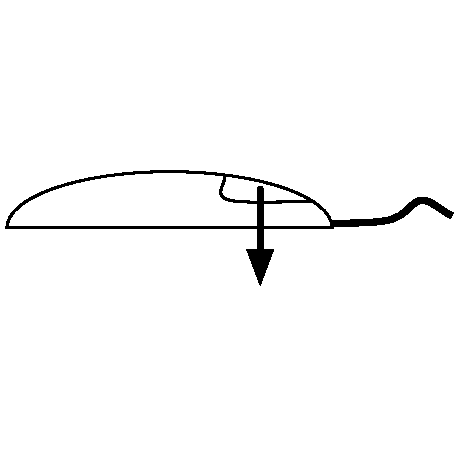
\includegraphics[origin=c, width=3.5cm]{img/button-force-mouse.pdf} 
}
\hspace{1cm} \subfigure[Pressing a stylus button is likely to cause
  accidental pen tip movement.] {
    \label{fig:button-force-pen}
    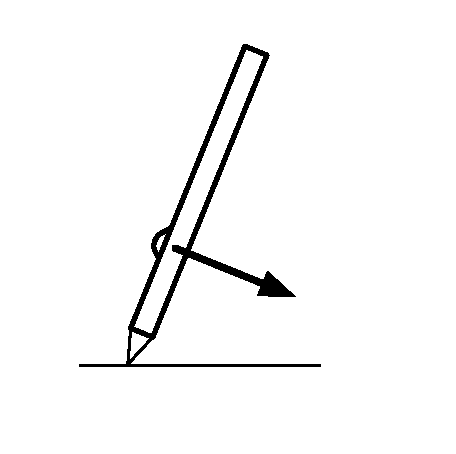
\includegraphics[origin=c, width=3.5cm]{img/button-force-pen.pdf}
}
\caption{The force required to press a mouse button compared with a
  stylus button.}
\label{fig:button-force}
\end{figure}

Some styluses have buttons. While buttons are an indispensable part of
a mouse, they are often difficult to use on the barrel of a
pen~\cite{plimmer-pen-usability}. The force of a \textit{mouse} button
click is orthogonal to the device's plane of use and has negligible
effect on target accuracy. However, pressing buttons on a
\textit{stylus} can move the tip of the pen, making it difficult to
press the button while pointing at particular objects (see
Figure~\ref{fig:button-force}). Further, pressing a button on a
computer stylus usually requires the user to adjust the pen in
hand. This action may be distracting and uncomfortable for long term
use.

\section{Large displays for drawing}

Groups of people often gather around traditional whiteboards to
brainstorm or exchange ideas. They draw pictures and diagrams,
maintain lists of text, and so on.  Whiteboards are also effective for
leaving asynchronous messages in the physical workspace where
co-workers can see them. People sometimes photograph whiteboards or
scan pages of sketches in order to record works-in-progress.

Electronic whiteboards such as the SmartBoard or those produced by
PolyVision more readily afford interactive usage than ordinary
whiteboards. For example, collaborative systems such as
Colab~\cite{stefik-colab} and Tivoli~\cite{pedersen-tivoli} support
meetings as people maintain checklists or collaboratively
draw. Systems can dynamically change their displays as people interact
with them, resizing or moving objects, or checking items in a
list~\cite{mynatt-flatland}. Large displays let more people have
simultaneous access to the drawing surface, which presents challenges
in sensing, and distinguishing between different users' pens.

Large displays have historically lacked portability, requiring a good
deal of time to install and calibrate. However, Lee recently
demonstrated a portable approach for projecting images on large
surfaces such as walls or tables, shown in
Figure~\ref{fig:lee-display}~\cite{lee-3d-infrared-pen}. The projector
emits patterns of time-multiplexed visible and infrared light. The
infrared light is decoded by sensors, providing a host computer with
fast and accurate location detection. The system uses sensors embedded
in the display surface to calculate the surface size and orientation
relative to the projector. Sensors may also be embedded in objects
such as pens, enabling alternate methods of user input. Equipping a
pen with a focusing lens allows it to become a short-distance pointing
device as in
Figure~\ref{fig:lee-display-2}~\cite[p. 62]{lee-projector-thesis}.

\begin{figure}
\centering
\subfigure[]
{
    \label{fig:lee-display-1}
    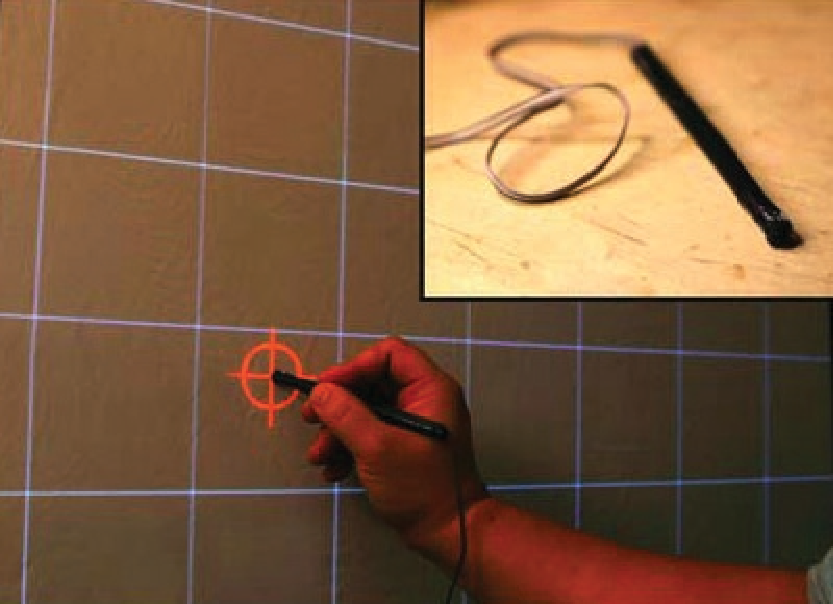
\includegraphics[origin=c, width=5cm]{img/lee-display-1.pdf}
}
\subfigure[]
{
    \label{fig:lee-display-2}
    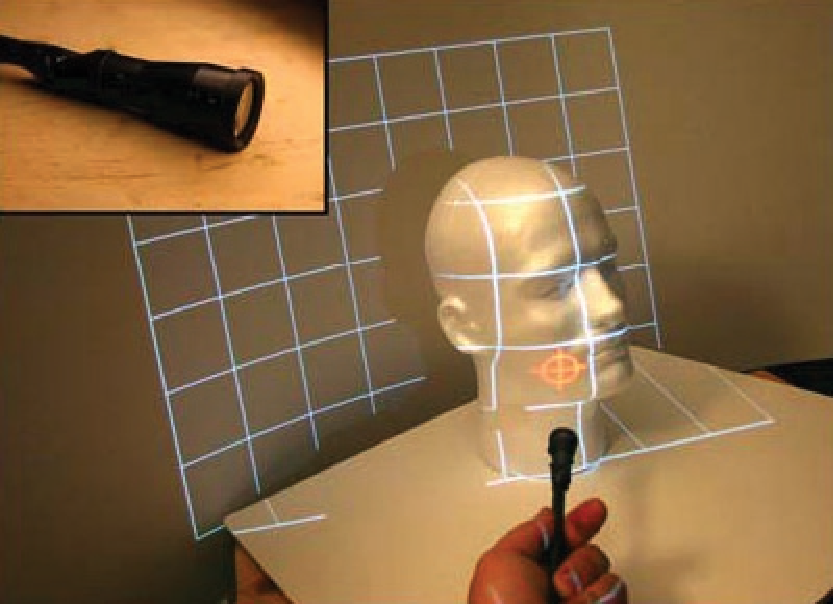
\includegraphics[origin=c, width=5cm]{img/lee-display-2.pdf}
}

\caption{Lee's portable projection approach enables detection of
  drawing surface size and orientation as well as pen input. This is
  effective on flat surfaces as in \subref{fig:lee-display-1} or
  curved surfaces as in \subref{fig:lee-display-2}.}

\label{fig:lee-display}
\end{figure}

At least two methods for capturing marks on ordinary whiteboards
utilize physical ink-like markers. The first uses traditional markers
whose activity can be detected by nearby sensors or cameras as the
user works, such as the Mimio commercial system. Whiteboard markers
are placed in sleeves whose position is calculated by the system
hardware.  Ju \textit{et. al} used a Mimio in the
WorkspaceNavigator~\cite{ju-navigator}.  PARC's
ZombieBoard~\cite{moran-collage-zombie,saund-zombie} used the second
method: scanning the whiteboard optically using a still camera. The
ZombieBoard enabled users to interact with the computer by drawing
special symbols. For example, users could delimit a region of the
whiteboard to be scanned by drawing its boundary. To invoke the scan,
the user would draw a button on the region boundary and draw an X or
check mark inside.

